\documentclass[12pt]{article}
\usepackage[utf8]{inputenc}
\usepackage{hyperref}
\usepackage{listings}
\usepackage{xcolor}
\usepackage{geometry}
\usepackage{graphicx} % For including graphics
\usepackage{minted} % For advanced code listings
\usepackage{listings-solidity}  % Include Solidity highlighting

% Define a custom minted style (optional)
\usemintedstyle{colorful} % You can choose from various styles like 'monokai', 'tango', 'colorful', etc.

% Custom color setup
\definecolor{bashtextcolor}{RGB}{0, 0, 0} % Define black color

% Define a new command for inline code using minted
\newcommand{\codeinline}[1]{\mintinline{text}{#1}}

\geometry{a4paper, margin=1in}

\title{Smart Contracts Exercise 04: \\ Unbreakable Vault}
\author{}
\date{}

% Define a new command for inline code with a dark background
\newcommand{\codeblack}[1]{%
  \texttt{\colorbox{black!7}{\textcolor{black}{#1}}}%
}

% Define a new command for inline code with a dark background
\newcommand{\codegrey}[1]{%
  \texttt{\colorbox{black!4}{\textcolor{black}{#1}}}%
}

% Define custom colors (optional)
\definecolor{myURLColor}{RGB}{0, 102, 204} % Example: A shade of blue

\hypersetup{
    colorlinks=true,        % Enable colored links
    linkcolor=blue,         % Color for internal links (e.g., \ref, \cite)
    citecolor=blue,         % Color for citations
    filecolor=magenta,      % Color for file links
    urlcolor=myURLColor     % Color for external URLs
}

% Define a style for code listings
\lstdefinestyle{mystyle}{
    backgroundcolor=\color{lightgray!20},   
    commentstyle=\color{green!50!black},
    keywordstyle=\color{blue},
    numberstyle=\tiny\color{gray},
    stringstyle=\color{red},
    basicstyle=\ttfamily\footnotesize,
    breakatwhitespace=false,         
    breaklines=true,                 
    captionpos=b,                    
    keepspaces=true,                 
    numbers=left,                    
    numbersep=5pt,                  
    showspaces=false,                
    showstringspaces=false,
    showtabs=false,                  
    tabsize=2
}

\lstset{style=mystyle}
% Adding package for header and footer
\usepackage{fancyhdr}
\pagestyle{fancy}

% Define header and footer
\fancyhf{} % Clear current settings
\fancyhead[L]{Smart Contracts Exercise 04} % Left header
\fancyhead[R]{\thepage} % Right header with page number

\renewcommand{\headrulewidth}{0.4pt} % Line below header
% \renewcommand{\footrulewidth}{0.4pt} % Line above footer

\begin{document}

\maketitle
\section{Introduction}
In this exercise, you will be tasked with breach several vaults, one by one. You will gain familiarity with the JavaScript library \href{https://docs.ethers.org/v6}{Ethers.js}, which is designed to facilitate interaction with the Ethereum blockchain and its ecosystem. We will also demonstrate how to work in \href{https://remix.ethereum.org/}{Remix IDE}, an open-source development environment accessible through a web browser. Additionally, you will learn about blockchain data transparency, storage, randomness pattern and the differences between \texttt{msg.sender} and \texttt{tx.origin}.

\subsection*{Prerequisites}

Ensure that you have already installed the following on your system:

\begin{itemize}
    \item \textbf{Node.js} - \url{https://nodejs.org/en/}
    An open-source, cross-platform, back-end JavaScript runtime environment that runs on the V8 engine and executes JavaScript code outside a web browser. 
    \item \textbf{NPM}: Node Package Manager, which comes with Node.js.
\end{itemize}

Open your terminal and run the following commands to verify the installations:

\begin{minted}[bgcolor=gray!5, fontsize=\footnotesize]{bash}
$ node -v
$ npm -v
\end{minted}

Both commands should return the installed version numbers of Node.js and NPM respectively. Node.js provides the runtime environment required to execute JavaScript-based tools like Hardhat, while NPM is used to manage the packages and dependencies needed for development. It is recommended that you use NPM 7 or higher.

For the purposes of this exercise, you will need an Infura API key and a configured wallet. If you do not have this set up yet, we recommend going through the Smart Contracts Exercise 01: Hello, Blockchain World! where everything is explained. Ensure that configuration variables are set for your Hardhat projects. You can verify this by running:

\begin{minted}[bgcolor=gray!5, fontsize=\footnotesize]{bash}
$ npx hardhat vars get INFURA_API_KEY
$ npx hardhat vars get SEPOLIA_PRIVATE_KEY
\end{minted}



\subsection*{Project Set Up}

To get started, visit the following \href{https://gitlab.fel.cvut.cz/radovluk/smart-contracts-exercises/-/tree/main/04-Unbreakable-Vault/task/task-code}{GitLab repository} and clone it to your local machine. This repository contains a template in which you will complete this exercise. After you clone the repository, start with the following command within your project folder:

\begin{minted}[bgcolor=gray!5, fontsize=\footnotesize]{bash}
$ npm install
\end{minted}
This will install all the necessary dependencies for the project. Your implementation will be in the \texttt{contracts} and \texttt{test} folders.
There will be multiple vaults in this exercise that you need to breach, each one having a separate test. To see if you have completed the task successfully, run \texttt{npm run vaultXX} where \texttt{XX} is the number of the vault you are trying to breach. For example, to test the first vault, run:
\begin{minted}[bgcolor=gray!5, fontsize=\footnotesize]{bash}
$ npm run vault01
\end{minted}
To run all tests at once, run:
\begin{minted}[bgcolor=gray!5, fontsize=\footnotesize]{bash}
$ npx hardhat test
\end{minted}

\section{Task: Breach the Vaults}
\subsection*{Vault01: A Password Password}
The first vault is quite straightforward. To complete this challenge, you need to call the \texttt{breachVault} function with the correct password and become the \texttt{lastSolver}. Implement your solution in \texttt{test/Vault01.js}. Do not alter the contract code. Use only the \texttt{player} account to breach the vault.

\begin{lstlisting}[language=Solidity]
  // SPDX-License-Identifier: MIT
  pragma solidity ^0.8.28;
  
  contract Vault01 {
      address public lastSolver;
  
      function breachVault(uint256 _password) public returns (bool) {
          require(
              _password == uint256(keccak256("password")),
              "Incorrect password"
          );
          lastSolver = tx.origin;
          return true;
      }
  }  
\end{lstlisting}

\medskip
\noindent
Sources you might want to use:
\begin{itemize}
  \item \href{https://docs.ethers.org/v6/api/hashing/}{https://docs.ethers.org/v6/api/hashing/}
  \item \href{https://docs.soliditylang.org/en/latest/}{https://docs.soliditylang.org/en/latest/}
\end{itemize}

\medskip
\noindent
Verify your solution with:
\begin{minted}[bgcolor=gray!5, fontsize=\footnotesize]{bash}
  $ npm run vault01
\end{minted}

\subsubsection*{Remix IDE}

In this exercise, each individual task is also available in Remix IDE. Remix is a versatile tool that requires no installation, promotes rapid development, and offers a wide range of plugins with intuitive GUIs created by Ethereum foundation. It is available as both a web application and a desktop application. The purpose of this is to familiarize you with the basic operations in this program and to facilitate your interaction with smart contracts.

\medskip
\noindent
\href{https://remix.ethereum.org/?#activate=solidity&url=https://github.com/radovluk/unbreakable-vault/contracts/Vault01.sol&lang=en&optimize=false&runs=200&evmVersion=null&version=soljson-v0.8.28+commit.7893614a.js}{Vault01 in Remix IDE}

\medskip
\noindent
How to get started with Remix:
\begin{itemize}
  \item \href{https://www.youtube.com/watch?v=vH8T3In6ZkE&t=7s&ab_channel=EatTheBlocks}{Getting Started With Remix (Solidity) in 2 mins}
  \item \href{https://remix-ide.readthedocs.io/en/latest/}{https://remix-ide.readthedocs.io/en/latest/}
\end{itemize}

\subsection*{Vault02: Packet Sender}

There is nothing new here, the previous hints are enough for you to break into this vault! Solve the challenge in \texttt{test/Vault02.js}.

\begin{lstlisting}[language=Solidity]
// SPDX-License-Identifier: MIT
pragma solidity ^0.8.28;
 
contract Vault02 {
    address public lastSolver;
 
    function breachVault(uint256 _password) public returns (bool) {
        require(
            _password == uint256(keccak256(abi.encodePacked(msg.sender))),
            "Incorrect password"
        );
        lastSolver = tx.origin;
        return true;
    }
}
\end{lstlisting}

\medskip
\noindent
\href{https://remix.ethereum.org/?#activate=solidity&url=https://github.com/radovluk/unbreakable-vault/contracts/Vault02.sol&lang=en&optimize=false&runs=200&evmVersion=null&version=soljson-v0.8.28+commit.7893614a.js}{Vault02 in Remix IDE}

\subsection*{Vault03: Origins}

In the Ethereum network, there are two main types of accounts:

\begin{itemize}
  \item Externally Owned Accounts (EOAs)
  \item Smart Contract Accounts (SCAs)
\end{itemize}
EOAs are managed by private keys, SCAs are governed by smart contract code.

\noindent
To breach the third vault, you need to understand the difference between \texttt{msg.sender} and \texttt{tx.origin}. The key distinction is that \texttt{tx.origin} always refers to the original external account that initiated the transaction, while \texttt{msg.sender} can be any contract or account that called the current function. As illustrated in the graph below (see Figure~\ref{fig:msg.sender}), smart contracts can call other smart contracts, but only an externally owned account can initiate a transaction and forward the gas. It is important to never use \texttt{tx.origin} for authentication. For this challenge, you cannot implement the solution directly in \texttt{test/Vault03}. Instead, you need to use a proxy contract. Implement your solution in \texttt{contracts/AttackVault03.sol}.

\begin{figure}[h!]
  \centering
  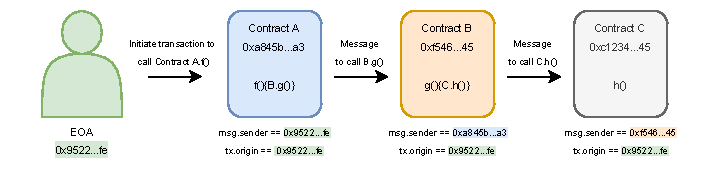
\includegraphics[width=0.95\textwidth]{msg.sender.pdf}
  \caption{msg.sender vs tx.origin}
  \label{fig:msg.sender}
\end{figure}

\begin{lstlisting}[language=Solidity]
// SPDX-License-Identifier: MIT
pragma solidity ^0.8.28;

contract Vault03 {
    // Address of the last person who solved the challenge
    address public lastSolver;

    function breachVault() public returns (bool) {
        require(msg.sender != tx.origin,
            "Caller must not be the transaction origin"
        );
        lastSolver = tx.origin;
        return true;
    }
}
\end{lstlisting}

\medskip
\noindent
\href{https://remix.ethereum.org/?#activate=solidity&url=https://github.com/radovluk/unbreakable-vault/contracts/Vault03.sol&lang=en&optimize=false&runs=200&evmVersion=null&version=soljson-v0.8.28+commit.7893614a.js}{Vault03 in Remix IDE}

\medskip
\noindent
Optional deep dive:
\href{https://eips.ethereum.org/EIPS/eip-4337}{EIP 4337} is a proposal that aims to enable smart contract-like functionality for all accounts, effectively eliminating the distinction between Externally Owned Accounts and Smart Contract Accounts. This would allow for more advanced and flexible control over account operations, including features like gas sponsorship, multi-signature authentication, and custom transaction logic.

\subsection*{Vault04: Pseudo-Random Trap}

Generating a random number in Ethereum can be tricky. The Ethereum Virtual Machine executes smart contracts in a deterministic environment, ensuring consistent outputs for identical inputs. Solidity does not provide anu function that generate random numbers. To work around this, some developers use pseudo-random number generators (PRNGs) based on \href{https://docs.soliditylang.org/en/latest/cheatsheet.html\#block-and-transaction-properties}{block properties} like:

\begin{itemize}
    \item \texttt{blockhash(uint blockNumber)}: Hash of a recent block.
    \item \texttt{block.number}: Current block number.
    \item \texttt{block.timestamp}: Block timestamp (Unix epoch).
\end{itemize}

\noindent
The problem is, that block proposers might attempt to delay transactions that do not yield the desired outcome. This issue is particularly relevant for transactions involving bigger amounts of money (more than the staking reward). It is potentially predictable and generally not recommended.

\subsubsection*{Solution with Oracles} Oracles are typically used to access external data from outside the blockchain. Additionally, oracles can provide verifiable random numbers. However, they come with limitations such as high gas costs and dependency on third parties (the oracle owner can manipulate the data). We will learn more about oracles in future exercises.

\subsubsection*{Commit and Reveal Scheme} Another solution might be commit and reveal scheme. The proccess involves two steps:
\begin{enumerate}
    \item \textbf{Commit}: Users (more than one) hash their random number concatenated with a secret value. They commit to this number by publishing the hash to the smart contract.
    \item \textbf{Reveal}: Users reveal their random number and the secret value. The smart contract verifies the hash and calculates the random number from these commits:
    \[
    \left( \sum_{i=1}^{n} r_i \right) \bmod N
    \]
    where $r_i$ is the random number from user $i$ and $N$ is the number of users.
\end{enumerate}
\noindent
A potential limitation is that it requires user interaction, and users can withhold their reveals.

\begin{figure}[H]
    \centering
    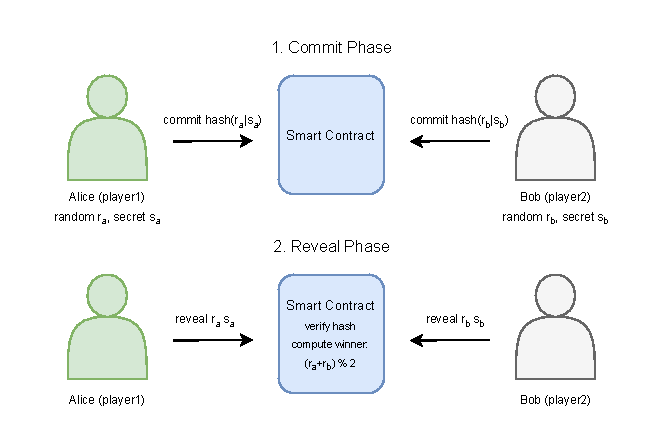
\includegraphics[width=0.85\textwidth]{commit-reveal.pdf}
    \caption{Commit and reveal scheme}
    \label{fig:commit-reveal}
\end{figure}

\medskip
\noindent
For this vault, you will need a proxy contract as well. Implement your solution in the \texttt{contracts/AttackVault04.sol} file.

\begin{lstlisting}[language=Solidity]
    // SPDX-License-Identifier: MIT
    pragma solidity ^0.8.28;
    
    contract Vault04 {
        address public lastSolver;
    
        function breachVault(uint256 guess) public returns (bool) {
            require(
                guess ==
                    uint256(
                        keccak256(
                            abi.encodePacked(
                                blockhash(block.number - 1),
                                block.timestamp
                            )
                        )
                    ) % 100,
                "Incorrect guess"
            );
            lastSolver = tx.origin;
            return true;
        }
    }
\end{lstlisting}

\medskip
\noindent
\href{https://remix.ethereum.org/?#activate=solidity&url=https://github.com/radovluk/unbreakable-vault/contracts/Vault04.sol&lang=en&optimize=false&runs=200&evmVersion=null&version=soljson-v0.8.28+commit.7893614a.js}{Vault04 in Remix IDE}

\subsection*{Vault05: Fortune Teller}

This vault cannot be opened without a crystal ball. Or can it? Implement your solution in the \texttt{test/Vault05.sol} file. Look for hints here: \href{https://docs.soliditylang.org/en/latest/units-and-global-variables.html}{Units and global variables in Solidity}.

\begin{lstlisting}[language=Solidity]
    // SPDX-License-Identifier: MIT
    pragma solidity ^0.8.28;
    
    contract Vault05 {
        address public lastSolver;
        uint256 private guess;
        uint256 private lockInBlockNumber;
    
        function lockInGuess(uint256 _guess) public {
            guess = _guess;
            lockInBlockNumber = block.number;
        }
    
        function breachVault() public returns (bool) {
            require(block.number > lockInBlockNumber, "Wait for the next block");
            require(
                guess == uint256(blockhash(lockInBlockNumber)) % 100,
                "Incorrect guess"
            );
            lastSolver = tx.origin;
            return true;
        }
    }
    
\end{lstlisting}

\medskip
\noindent
\href{https://remix.ethereum.org/?#activate=solidity&url=https://github.com/radovluk/unbreakable-vault/contracts/Vault05.sol&lang=en&optimize=false&runs=200&evmVersion=null&version=soljson-v0.8.28+commit.7893614a.js}{Vault05 in Remix IDE}

\subsection*{Vault06: Explorer}

EVM can store data in three different places: storage, memory, and stack.

\begin{itemize}
\item \textbf{Storage} keeps data between function calls and is persistent for every smart contract. It is the most expensive type of memory in terms of gas cost. We can think of storage as a hard drive. State variable are saved in storage by default.

\item \textbf{Memory} is a temporary storage location for data. Once execution is completed, memory is cleared for the next execution. It is comparable to RAM.

\item \textbf{Stack} EVM is a stack machine rather than a register machine; all computations are done in the data region called the stack. It has a strict size limit (1024 slots), meaning complex operations often require \texttt{memory} or \texttt{storage}.

\end{itemize}

\noindent
It's important to note that marking a variable as private only restricts access from other contracts. Private state variables and local variables remain publicly accessible. For this task, there is already a deployed contract on the Sepolia testnet. You can find the contract address and the source code below. Implement your solution in the \texttt{test/Vault06.js} file. The address of the deployed contract is \texttt{0xA3a763bF62550511A0E485d6EB16c98937609A32}.

\begin{lstlisting}[language=Solidity]
  // SPDX-License-Identifier: MIT
  pragma solidity ^0.8.28;
  
  contract Vault06 {
      address public lastSolver;
      string private password;
  
      constructor(string memory _password) {
          password = _password;
      }
  
      function breachVault(string memory _password) public returns (bool) {
          require(
              keccak256(abi.encodePacked(password)) ==
                  keccak256(abi.encodePacked(_password)),
              "Incorrect password"
          );
          lastSolver = tx.origin;
          return true;
      }
  }
\end{lstlisting}

\medskip
\noindent
\textbf{Hint:} For this challenge, you can find the solution just by closely inspecting the contract on: \href{https://sepolia.etherscan.io/address/0xA3a763bF62550511A0E485d6EB16c98937609A32}{Vault06 on Sepolia Etherscan}

\medskip
\noindent
You can also interact with the contract directly from the Remix IDE if you connect it to your MetaMask wallet, change the environment to "Injected Provider - MetaMask" and use the "Load contract from address" function.

\medskip
\noindent
\href{https://remix.ethereum.org/?#activate=solidity&url=https://github.com/radovluk/unbreakable-vault/contracts/Vault06.sol&lang=en&optimize=false&runs=200&evmVersion=null&version=soljson-v0.8.28+commit.7893614a.js}{Vault06 in Remix IDE}

\subsection*{Vault07: You Shall Not Pass!}

\noindent
In this exercise, you will not be able to find the solution just by inspecting Etherscan as you did in the previous exercise. Instead, you will need to decode the storage yourself. You can find the necessary functions here: \href{https://docs.ethers.org/v6/api/providers/}{https://docs.ethers.org/v6/api/providers/}. Implement your solution in the \texttt{test/Vault07.js} file. The address of the deployed contract is \texttt{0xa81C96B2216eDFfF8945e371dd581D13f8ECfbAD}.

\begin{lstlisting}[language=Solidity]
    // SPDX-License-Identifier: MIT
    pragma solidity ^0.8.28;
    
    contract Vault07 {
        address public lastSolver;
        uint8 private small1 = 42;
        uint16 private small2 = 999;
        bool private isActive = true;
        uint256 private big1 = 1337;
        bytes32 private hashData = keccak256(abi.encode("You Shall Not Pass"));
        uint256 private big2 = 0xDEADBEEF;
        string private password;
    
        constructor(string memory _password) {
            password = _password;
        }
    
        function breachVault(bytes32 _password) public returns (bool) {
            require(
                keccak256(abi.encodePacked(password, msg.sender)) == _password,
                "Incorrect password"
            );
            lastSolver = tx.origin;
            return true;
        }
    }
\end{lstlisting}

\medskip
\noindent
\href{https://remix.ethereum.org/?#activate=solidity&url=https://github.com/radovluk/unbreakable-vault/contracts/Vault07.sol&lang=en&optimize=false&runs=200&evmVersion=null&version=soljson-v0.8.28+commit.7893614a.js}{Vault07 in Remix IDE}

\medskip
\noindent
\textbf{Hint:} \href{https://medium.com/@flores.eugenio03/exploring-the-storage-layout-in-solidity-and-how-to-access-state-variables-bf2cbc6f8018}{Exploring the Storage Layout in Solidity and How to Access State Variables}

\end{document}
